\chapter{Resistance of a Conductor}

\section{Aim}
To find the relationship between the resistance of a conductor and its length

\section{Background Information}
All conductors have resistance. This resistance may depend on many factors including the shape and properties of the material as well as its temperature. It is important to isolate each factor to determine the exact relationship between it and the resistance so that resistance calculations can be simplified for manufacturing purposes. In this experiment, we focus on the shape and determine what happens if the length of the conductor changes. 

\section{Materials}
Dry cell size D (1.5 V), connecting wires, potential meter\slash meter bridge, ammeter, crocodile clip. 

\section{Procedure}
\begin{enumerate}
\item Connect a dry cell, $E$, with an ammeter, $A$, and one end of a meter bridge.
\item Attach a connecting wire to the other end of the dry cell and the wire on the meter bridge at the 20 cm mark, using a crocodile clip as seen in Figure \ref{fig:resistance-conductor-1}. 
\item Record the current, $I$, on the ammeter and the distance $L$ which the meter bridge wire is in the circuit. 
\item Repeat steps 2-3 for the length ($L$) of 40, 60, and 80 cm. 
\item Tabulate your results for current ($I$) and length ($L$).
\end{enumerate}

\begin{figure}[h!]
\centering
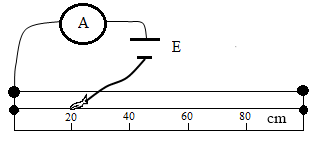
\includegraphics[width=10cm]{./img/resistance-conductor-1.png}
\caption{Resistance of a Conductor practical setup}
\label{fig:resistance-conductor-1}
\end{figure}

\section{Analysis and Interpretation}
\begin{enumerate}
\item Compute the values of resistance for each case.
\item Plot a graph of resistance ($R$) versus length ($L$).
\item What is the nature of the graph?
\item Find the slope and vertical intercept. What does the vertical intercept represent?
\end{enumerate}

\section{Conclusion}
What is the relationship between the length of the conductor and its resistance?

\section{Questions for Discussion}
\begin{enumerate}
\item Do you think the resistance of a conducting wire also depends on its cross-sectional area? Explain.
\item What are the errors in this experiment and how do they affect your results?
\item What would be the resistance of the meter bridge wire if it were 2 meters long?
\end{enumerate}

\section{Reflection and Self Assessment}
\begin{enumerate}
\item Is there anything you do not understand in this experiment? If so what is it and in what ways can you increase your understanding?
\item How might an electrician need this knowledge to produce a proper circuit?
\end{enumerate}